\begin{definition}[Neighborhood] \leavevmode \\
    Let $(X,d)$ be a metric space, $p \in X, ~\epsilon > 0$.
    $$N_\epsilon (p) = \{x\in X : d(p,x) < \epsilon\}$$
    is the neighborhood of radius $\epsilon$. This is also known as an open ball of radius $\epsilon$ centered at $p$.
\end{definition}

\begin{note}
    $x\in N_\epsilon (p) \iff d(p,x) < \epsilon$
\end{note}

\begin{example}
    $(\mathbb{R}, d),~~ d(x,y) = |x-y|$.
    Let $p \in \mathbb{R}, ~\epsilon > 0.$
    \begin{align*}
        N_\epsilon (p) &= \{x \in \mathbb{R} : d(x,p) < \epsilon\} \\
        &=\{x \in \mathbb{R} : |x - p| < \epsilon\} \\
        &= \{x \in \mathbb{R} : p -\epsilon < x < p + \epsilon\} \\
        &=(p-\epsilon, p + \epsilon)
    \end{align*}
    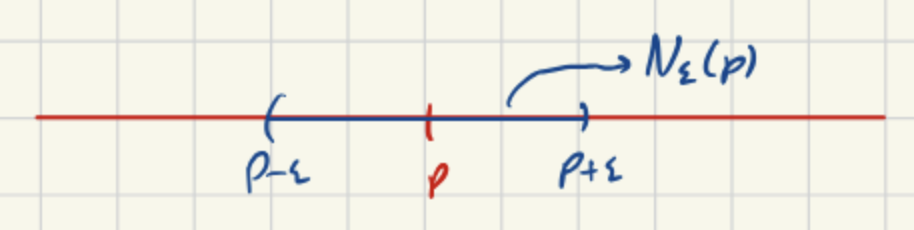
\includegraphics[width=.50\linewidth, center]{/Users/josiahvillarante/GradSchool/Grad-School-Notes/Math230A/Lecture/CH2/images/neighborhood in R.png}
\end{example}

\begin{example}
    $(\mathbb{R}^2, d), ~~d((a,b),(x,y)) = \sqrt{(a-x)^2 + (b-y)^2}$.
    Let $(a,b) \in \mathbb{R}^2, ~\epsilon > 0$.
    \begin{align*}
        N_\epsilon(a,b) &= \{(x,y) \in \mathbb{R}^2 : d\big((x,y),(a,b)\big) < \epsilon\} \\ &= \{(x,y) \in \mathbb{R}^2 : \sqrt{(x-a)^2+(y-b)^2} < \epsilon \} \\ &= \{(x,y) \in \mathbb{R}^2 : (x-a)^2 + (y-b)^2 < \epsilon^2 \}
    \end{align*}
    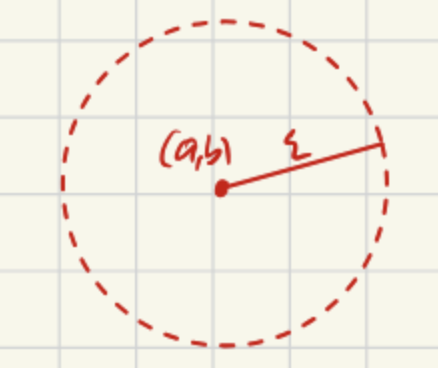
\includegraphics[width=.30\linewidth, center]{/Users/josiahvillarante/GradSchool/Grad-School-Notes/Math230A/Lecture/CH2/images/neighborhood in R2.png}
\end{example}

\begin{example}
     $(\mathbb{R}^2, d), ~~d((a,b),(x,y))= |a-x|+|b-y|.$ $$N_1(0,0) = \{(x,y) \in \mathbb{R}^2 : d\big((x,y),(0,0)\big) < 1\} = \{(x,y) \in \mathbb{R}^2 : |x| + |y| < 1\}$$
     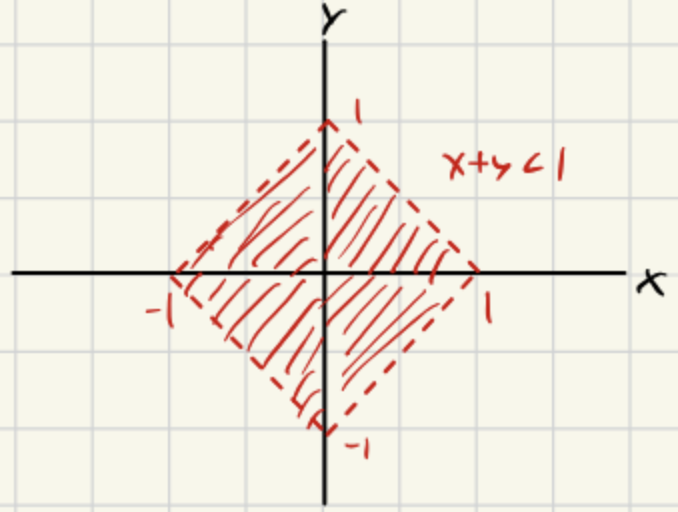
\includegraphics[width=.30\linewidth, center]{/Users/josiahvillarante/GradSchool/Grad-School-Notes/Math230A/Lecture/CH2/images/neighborhood diamond.png}
\end{example}

\begin{example}
    $(\mathbb{R}, d) ~~d(x,y) = \begin{cases}1 &\text{if } x\not = y \\ 0 &\text{if } x=y \end{cases}$
    Let $p \in \mathbb{R}$ and $\epsilon > 0$. What is $N_\epsilon (p)$?
    \begin{description}
        \item[Case 1: $\epsilon \leq 1$] Note that if $d(x,p) < \epsilon \leq 1$, then $d(x,p) < 1$ and so $d(x,p) = 0$. Hence $x=p$.
        $$N_\epsilon (p) = \{x \in \mathbb{R} : d(x,p) < \epsilon \}$$
    \end{description}
    
\includegraphics[width=.30\linewidth, center]{/Users/josiahvillarante/GradSchool/Grad-School-Notes/Math230A/Lecture/CH2/images/neighborhood discrete 1.png}
    
    \begin{description}
        \item[Case 2: $\epsilon > 1$] Clearly, for all $x\in \mathbb{R}, ~~d(x,p) \leq 1 < \epsilon$.
        So,
        $$N_\epsilon (p) = \{x \in \mathbb{R} : d(x,p) < \epsilon\} = \mathbb{R}$$
    \end{description}
    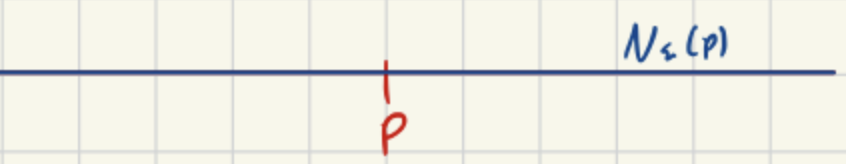
\includegraphics[width=.30\linewidth, center]{/Users/josiahvillarante/GradSchool/Grad-School-Notes/Math230A/Lecture/CH2/images/neighborhood discrete 2.png}
\end{example}

\begin{definition}[Limit Point, Isolated Point] \leavevmode \\
    Let $(X, d)$ be a metric space, $E \subseteq X$. A point $p\in X$ is said to be a limit point of $E$ if $$\forall \epsilon > 0 ~~N_\epsilon (p) \cap (E ~\backslash \{p\}) \not = \emptyset.$$The collection of all limit points of $E$ is denoted by $E'$. $$E'=\{p\in X : \forall \epsilon > 0, ~N_\epsilon (p)\cap (E ~\backslash \{p\}) \not = \emptyset\}.$$A point $p\in E$ is said to be an isolated point of $E$ if $p$ is not a limit point.
\end{definition}

\begin{note}
     $p$ is an isolated point of $E \iff p\in E$ and $p\not \in E'$
\end{note}

\begin{example}
    $(\mathbb{R}, d), ~~d(x,y) = |x-y|, ~~E=\{\frac{1}{n} : n \in \mathbb{N} \}$. Prove that $0 \in E'.$
    Note that $0 \not \in E$. Also recall that
    $$0 \not \in E' \iff \forall \epsilon > 0, ~N_\epsilon(0) \cap E \not = \emptyset.$$
    That is, we need to show that
    $$\forall \epsilon > 0 ~~~(-\epsilon, \epsilon)\cap E \not = \emptyset.$$
    Let $\epsilon > 0$ be given. By the Archimedean property of $\mathbb{R} ~~\exists m\in \mathbb{N}$ such that $\frac{1}{m} < \epsilon.$ Clearly, $\frac{1}{m} \in (-\epsilon, \epsilon) \cap E$. 

    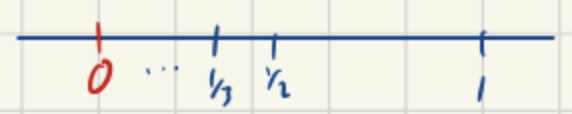
\includegraphics[width=.30\linewidth, center]{/Users/josiahvillarante/GradSchool/Grad-School-Notes/Math230A/Lecture/CH2/images/limit point 1.png}
\end{example}

\begin{remark}
    $p \in E' \iff$ there is a sequence of distinct points in $E$ that converges to $p$.
\end{remark}

\begin{example}
    $(\mathbb{R}, d), ~~d(x,y) = |x-y|, E=(1,2) \cup {5}$. Prove that $5$ is an isolated point of $E$.
    Since $5 \in E$, it is enough to show that $5 \not \in E'$. Recall that $5\not \in E' \iff \exists \epsilon > 0$ such that $(5 - \epsilon, 5 + \epsilon) \cap (1,2) = \emptyset$. Clearly, $\epsilon = 1$ does the job.
\end{example}

\begin{example}
    $(\mathbb{R}^2, d), ~~d\big((a,b),(x,y)\big) = \sqrt{(a-x)^2 + (b-y)^2}, E = \{(x,y) \in \mathbb{R}^2 : x^2 + y^2 = 4\}$. What is $E'?$
    $E' = (\text{the boundary circle})\cup E = \{(x,y), \in \mathbb{R}^2 : x^2 + y^2 \leq 4\}$.
    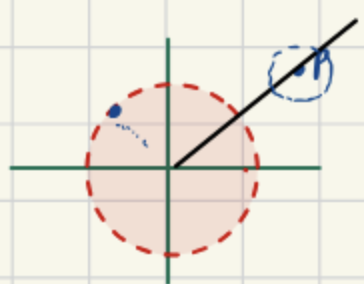
\includegraphics[width=.30\linewidth, center]{/Users/josiahvillarante/GradSchool/Grad-School-Notes/Math230A/Lecture/CH2/images/limit point 2.png}
    For example, if $(a,b)$ is such that $a^2 + b^2 > 4$, then $(a,b) \not \in E'$. Let $\delta = \frac{1}{2}(\sqrt{a^2 + b^2} - 2)$. Clearly, $N_\delta (p) \cap (E \backslash \{p\}) = \emptyset$.
\end{example}
